% Provenance (never printed): old terminale S material on the transformation of
% rocks in mountain belts and subduction zones (pressure, temperature, index
% minerals and the Al2SiO5 polymorphs, foliation, contact and regional
% metamorphism). Owner (Sync 0): metamorphism, lithostatic pressure, polymorph,
% index mineral/isograd/metamorphic grade, foliation/schistosity, contact and
% regional metamorphism/aureole. Blueschist and eclogite are g11.06's, the
% geotherm g11.03's, minerals and silicates g11.07's, the rock families, marble
% and slate Book 1's (g6), pressure physics': recalled, never redefined. The
% P-T diagram: figdata/grade-12/al2sio5.py (Holdaway and Mukhopadhyay 1993,
% Table 11; geotherms from Earle 7.3).
\chapter{Las rocas metamórficas}\label{ch:g12:metamorphic-rocks}

Una capa de fango se deposita en un fondo marino y se endurece hasta formar
una lutita. Entiérrala unos kilómetros y comprímela, y se convierte en una
pizarra, una roca que se separa en las láminas finas y planas de un tejado.
Entiérrala más hondo y a más temperatura, y sus diminutas escamas crecen hasta
formar micas brillantes, entre las que se hinchan granates rojos: un esquisto.
Más hondo y más caliente aún, sus minerales se ordenan en bandas claras y
oscuras: un gneis. Nada se ha fundido por el camino. El mismo fango, con los
mismos elementos químicos, se ha limitado a reconstruir sus minerales para
adaptarlos al lugar donde estaba. Leídos al revés, los minerales de una roca
metamórfica registran lo profundo y lo caliente que era ese lugar, y este
capítulo aprende a leerlos.
% ledger: earle:foliation, earle:settings

\begin{recall}
Las rocas se agrupan en tres familias ---ígneas, sedimentarias,
metamórficas--- y el ciclo de las rocas convierte unas en otras; el mármol se
forma a partir de la caliza y la pizarra a partir de la lutita, sin fundirse
(Libro 1, año 6). Un mineral es un sólido natural de composición química
definida y con una disposición ordenada de sus átomos; la mayoría de los
minerales de la corteza son \omterm{def:g11:minerals:silicate}{silicatos}
(el \cref{ch:g11:minerals}). Una \omterm{def:g11:lithosphere-asthenosphere:geotherm}{geoterma} es la curva de la temperatura frente
a la profundidad bajo un lugar; cerca de la superficie, la temperatura sube de
25 a \qty{30}{\celsius} por kilómetro (el \cref{ch:g11:lithosphere-asthenosphere}).
En una \omterm{def:g11:subduction-zones:subduction}{zona de subducción}, la \omterm{def:g11:ocean-ridges:oceanic-lithosphere}{corteza oceánica} arrastrada hacia abajo mientras
sigue fría se transforma en \omterm{def:g11:subduction-zones:eclogite}{esquisto azul} y luego en \omterm{def:g11:subduction-zones:eclogite}{eclogita} (el
\cref{ch:g11:subduction-zones}). La presión es una fuerza dividida por el área
sobre la que se ejerce; se mide en pascales, \qty{1}{Pa} = \qty{1}{N/m^2}.
\end{recall}
% ledger: usgs:metamorphic (Book 1 row), webmineral:formulas, earle:settings, earle:controls

\section{Transformadas en estado sólido}

\begin{definition}[Metamorfismo]\label{def:g12:metamorphic-rocks:metamorphism}
El \emph{metamorfismo}\index{metamorfismo} es la transformación de los
minerales y la \omterm{def:g11:igneous-rocks:texture}{textura} de una roca, en estado sólido, cuando se lleva a una
temperatura y una presión distintas de aquellas en las que se formó. La roca
en que se convierte es una roca metamórfica.
\end{definition}
% ledger: tulane:metamorphism, earle:controls

La roca de la que parte el \omterm{def:g12:metamorphic-rocks:metamorphism}{metamorfismo} es su \omterm{def:g10:soil-formation:weathering-profile}{roca madre}, las mismas palabras
que para la roca que hay bajo un suelo (el \cref{ch:g10:soil-formation}). El
\omterm{def:g12:metamorphic-rocks:metamorphism}{metamorfismo} empieza hacia los \qty{200}{\celsius}; por debajo, los lentos
cambios de un sedimento enterrado forman parte de su endurecimiento en roca.
Termina donde la roca empieza a fundirse: a partir de ahí, lo que ocurre es
ígneo. Entre esos límites, cada mineral solo es estable en un cierto
intervalo de temperatura y de presión. La mayoría de los \omterm{def:g10:soil-formation:clay}{minerales de la
arcilla}, por ejemplo, solo resisten hasta unos 150 o \qty{200}{\celsius}; por
encima, se transforman en micas. Cuando cambian las condiciones, los átomos de
los minerales inestables se reorganizan, grano a grano, en minerales que son
estables en las nuevas condiciones.
% ledger: tulane:metamorphism, earle:controls

Cuatro factores controlan el resultado. La \textbf{\omterm{def:g10:soil-formation:weathering-profile}{roca madre}} aporta los
elementos químicos: una caliza formada solo por calcita solo puede convertirse
en un mármol formado por calcita. La \textbf{temperatura} y la \textbf{presión} deciden qué
minerales son estables. Y el \textbf{agua}, presente en pequeñas cantidades
entre los granos, lleva iones disueltos de un grano al siguiente y acelera
las reacciones. El \omterm{def:g12:metamorphic-rocks:metamorphism}{metamorfismo} es lento: los minerales nuevos crecen alrededor
de un milímetro en un millón de años. Los procesos tectónicos que entierran
las rocas también son lentos, así que las reacciones suelen tener tiempo de
completarse.
% ledger: earle:controls

\subsection{El peso de las rocas de encima}

Una roca enterrada a una profundidad $z$ soporta el peso de toda la roca que tiene encima.

\begin{definition}[Presión litostática]\label{def:g12:metamorphic-rocks:lithostatic}
La \emph{presión litostática}\index{presion litostatica@presión litostática} a una
profundidad $z$ es la presión que ejerce sobre una roca el peso de la columna
de roca que tiene encima. Es la misma en todas las direcciones.
\end{definition}
% ledger: earle:controls (confining pressure, equal in all directions), tulane:metamorphism

\begin{proposition}[Presión litostática]\label{prop:g12:metamorphic-rocks:lithostatic}
Bajo una columna de roca de densidad uniforme $\rho$, la \omterm{def:g12:metamorphic-rocks:lithostatic}{presión litostática}
a la profundidad $z$ es
\[
  P = \rho g z ,
\]
donde $g$ es la aceleración de la gravedad; se desprecia la presión de la
atmósfera, de unos \qty{0.1}{MPa}.
\end{proposition}

\begin{proof}
Toma una columna vertical de roca de sección horizontal $A$, desde la
superficie hasta la profundidad $z$. Su volumen es $Az$, su masa $\rho A z$ y
su peso $\rho A z g$. Este peso descansa sobre el área $A$ del fondo de la
columna, así que la presión allí es $P = \rho A z g / A = \rho g z$.
\end{proof}

Con la densidad media de la \omterm{def:g12:continental-crust:continental-crust}{corteza continental}, $\rho = \qty{2830}{kg/m^3}$,
y $g = \qty{9.81}{m/s^2}$, la presión aumenta $\rho g = 2830 \times 9.81
\approx \qty{27800}{Pa}$ por metro, es decir, unos \qty{27.8}{MPa} por
kilómetro. En la base de una corteza de \qty{35}{km} de espesor alcanza
\[
  P = 2830 \times 9.81 \times \num{35000} \approx \qty{9.7e8}{Pa} \approx
  \qty{0.97}{GPa},
\]
alrededor de \qty{1}{GPa}: casi diez mil veces la presión de la atmósfera al
nivel del mar. Las presiones se leen a menudo al revés, como profundidades:
\qty{1}{GPa} se alcanza a $\num{e9}/(2830 \times 9.81) \approx \qty{36}{km}$
de profundidad.
% values: P_35km_gpa 0.97168, dPdz_mpa_per_km 27.762, z_1gpa_km 36.02 (al2sio5.py)
% ledger: cm95:crust; Book 1: ussa76:sea-level (101 325 Pa, g0 = 9.80665 m/s2)

El peso de las rocas empuja por igual desde todos los lados. En un cinturón
montañoso, las placas añaden un empuje en una dirección: la roca se comprime
más por los lados que desde arriba. Esta presión \emph{dirigida} no cambia
qué minerales son estables, pero sí cómo se disponen, como muestra la
\cref{sec:g12:metamorphic-rocks:foliation}.
% ledger: earle:controls (directed pressure), earle:foliation

\section{Minerales índice y grado}

\subsection{Tres minerales con una misma fórmula}

\begin{definition}[Polimorfo]\label{def:g12:metamorphic-rocks:polymorph}
Dos minerales son \emph{polimorfos}\index{polimorfo} cuando tienen la misma
composición química pero estructuras cristalinas distintas: los mismos
átomos, dispuestos de otra manera.
\end{definition}
% ledger: earle:controls

Tres minerales comparten la fórmula \ce{Al2SiO5}: la cianita, la andalucita y
la sillimanita. Cada uno es estable en su propio intervalo de temperatura y
de presión, medido en el laboratorio manteniendo cristales a una temperatura y
una presión elegidas y observando qué \omterm{def:g12:metamorphic-rocks:polymorph}{polimorfo} crece a costa del otro. La
cianita es la más densa de los tres,
\qty{3.61}{g/cm^3} frente a \qty{3.24}{g/cm^3} de la sillimanita y
\qty{3.15}{g/cm^3} de la andalucita: sus átomos están más apretados, y es la
que favorecen las presiones altas.
% ledger: earle:controls, hm93:triple, hm93:table11; Book 3: webmineral:polymorphs (densities)

\begin{omfigure}
\begin{tikzpicture}
\begin{axis}[omrecord, name=pt, scale only axis, width=0.62\linewidth, height=6.4cm,
  xmin=200, xmax=900, ymin=0, ymax=1.2, y dir=reverse,
  xlabel={temperatura (\unit{\celsius})}, ylabel={presión (\unit{GPa})},
  xtick={200,300,...,900}, ytick={0,0.2,...,1.2},
  yticklabel style={/pgf/number format/fixed, /pgf/number format/precision=1},
  axis y line*=left]
% computed in figdata/grade-12/al2sio5.py from Holdaway and Mukhopadhyay (1993), Table 11
\addplot[omDef, line width=0.9pt, densely dashed] table[x=T10, y=P_GPa] {figdata/out/grade-12-al2sio5-geotherms.dat};
\addplot[omMeth, line width=0.9pt, densely dashed] table[x=T30, y=P_GPa] {figdata/out/grade-12-al2sio5-geotherms.dat};
\addplot[omThm, line width=0.9pt, densely dashed] table[x=T50, y=P_GPa] {figdata/out/grade-12-al2sio5-geotherms.dat};
\addplot[black, line width=1.2pt] table[x=T, y=P_GPa] {figdata/out/grade-12-al2sio5-andky.dat};
\addplot[black, line width=1.2pt] table[x=T, y=P_GPa] {figdata/out/grade-12-al2sio5-kysil.dat};
\addplot[black, line width=1.2pt] table[x=T, y=P_GPa] {figdata/out/grade-12-al2sio5-andsil.dat};
\addplot[black, line width=1.2pt, dotted] table[x=T, y=P_GPa] {figdata/out/grade-12-al2sio5-andsilx.dat};
\addplot[only marks, mark=*, mark size=2pt, black] coordinates {(504.2,0.3758)};
\addplot[only marks, mark=o, mark size=2pt, line width=0.8pt, black] coordinates {(573.6,0.5216) (340.1,0.1833) (553.0,0.3015)};
\coordinate (ky) at (axis cs:370,0.55);
\coordinate (and) at (axis cs:470,0.12);
\coordinate (sil) at (axis cs:765,0.57);
\coordinate (tp) at (axis cs:504.2,0.3758);
\coordinate (g10) at (axis cs:415,1.0);
\coordinate (g30) at (axis cs:206,0.36);
\coordinate (g50) at (axis cs:895,0.355);
\end{axis}
\begin{axis}[scale only axis, width=0.62\linewidth, height=6.4cm, at={(pt.south west)}, anchor=south west,
  xmin=200, xmax=900, ymin=0, ymax=43.224, y dir=reverse, axis x line=none, axis y line*=right,
  axis line style={-}, ylabel={profundidad (\unit{km})}, ytick={0,5,...,40},
  every axis label/.append style={font=\small}, tick label style={font=\small}]
\end{axis}
\node[font=\small\bfseries] at (ky) {cianita};
\node[font=\small\bfseries] at (and) {andalucita};
\node[font=\small\bfseries] at (sil) {sillimanita};
\node[font=\scriptsize, text=omDef, anchor=west, inner sep=1pt] at (g10) {\qty{10}{\celsius/km}, zona de subducción};
\node[font=\scriptsize, text=omMeth!70!black, anchor=north west, inner sep=1pt, align=left] at (g30) {\qty{30}{\celsius/km},\\típica};
\node[font=\scriptsize, text=omThm, anchor=south east, inner sep=1pt] at (g50) {\qty{50}{\celsius/km}, zona volcánica};
\end{tikzpicture}

{\small Los campos de los tres \omterm{def:g12:metamorphic-rocks:polymorph}{polimorfos} de \ce{Al2SiO5}, con la presión
creciendo hacia abajo como la profundidad (escala de la derecha, para una
corteza de densidad \qty{2830}{kg/m^3}). Líneas negras: los límites medidos en
el laboratorio; los tres se cortan en el punto triple (punto negro),
\qty{504}{\celsius} y \qty{0.375}{GPa}. Discontinuas: tres \omterm{def:g11:lithosphere-asthenosphere:geotherm}{geotermas} que parten
de \qty{10}{\celsius} en la superficie; los círculos marcan dónde cruzan un
límite.}
\end{omfigure}
% values: triple_T 504.21, triple_P_gpa 0.37584, triple_z_km 13.538; crossings 30: 573.6 degC 18.79 km; 50: 340.1 degC 6.60 km, 553.0 degC 10.86 km (al2sio5.py)
% ledger: hm93:table11, hm93:triple, cm95:crust, earle:settings

El diagrama es un mapa de estabilidad. Cada punto es una temperatura y una
presión; cada campo es el \omterm{def:g12:metamorphic-rocks:polymorph}{polimorfo} que es estable allí. La cianita ocupa las
presiones altas, la andalucita las presiones bajas y las temperaturas
moderadas, la sillimanita las temperaturas altas. A lo largo de un límite, dos
\omterm{def:g12:metamorphic-rocks:polymorph}{polimorfos} son igual de estables, y en el punto triple, los tres. Los límites
no se conocen con exactitud: el punto triple tiene una incertidumbre de unos
\qty{20}{\celsius} y \qty{0.025}{GPa}, y las trazas de hierro en los cristales
desplazan la línea andalucita--sillimanita hasta \qty{20}{\celsius}.
% ledger: hm93:triple

\begin{method}[Leer un diagrama presión--temperatura]\label{met:g12:metamorphic-rocks:pt}
\begin{enumerate}
  \item Sitúa el punto de la roca: su temperatura en el eje horizontal, su
        presión en el vertical.
  \item Lee el campo en el que cae: el mineral estable allí.
  \item Convierte la presión en profundidad con $z = P/(\rho g)$, o léela en
        la escala de profundidad.
  \item Para un mineral hallado en una roca, lee al revés: la roca estaba en
        el campo de ese mineral cuando este cristalizó. Dos minerales que se
        formaron juntos, o un mineral que falta, acotan más el intervalo.
\end{enumerate}
\end{method}

\begin{example}[El límite cianita--sillimanita]\label{ex:g12:metamorphic-rocks:kysil}
A \qty{0.6}{GPa}, la cianita se transforma en sillimanita hacia los
\qty{611}{\celsius}. Esa presión se alcanza a $z = \num{0.6e9} / (2830
\times 9.81) \approx \qty{21.6}{km}$. Entre 600 y \qty{700}{\celsius}, el
límite sube \qty{0.209}{GPa}, es decir, $0.209/0.0278 \approx
\qty{7.5}{km}$ de profundidad: una roca \qty{7.5}{km} más profunda debe estar
unos \qty{100}{\celsius} más caliente para transformarse en sillimanita. Un
esquisto que contiene cianita pero no sillimanita y que cristalizó a
\qty{21.6}{km} estaba, por tanto, a menos de unos \qty{611}{\celsius}.
\end{example}
% values: kysil_T_at_6kbar 611, kysil_z_at_6kbar 21.612, kysil_slope 2.09 kbar per 100 degC, dPdz 27.762 MPa/km (al2sio5.py)

\subsection{Minerales índice e isógradas}

En un cinturón de rocas que empezaron todas como el mismo fango, los
minerales cambian de un lugar a otro, porque las rocas no se enterraron todas
a la misma profundidad ni se calentaron por igual.

\begin{definition}[Mineral índice; isógrada; grado metamórfico]\label{def:g12:metamorphic-rocks:index-mineral}
El \emph{grado metamórfico}\index{grado metamorfico@grado metamórfico} de una roca
es la intensidad del \omterm{def:g12:metamorphic-rocks:metamorphism}{metamorfismo} que ha sufrido, fijada por la temperatura y
la presión que alcanzó. Un \emph{mineral índice}\index{mineral indice@mineral índice}
es un mineral cuya primera aparición, en rocas de la misma composición
original, marca un grado dado. Una \emph{isógrada}\index{isograda@isógrada} es la
línea de un mapa (una superficie en el terreno) que une los lugares donde
aparece por primera vez un mineral índice: a lo largo de ella, las rocas han
alcanzado el mismo grado.
\end{definition}
% ledger: tulane:metamorphism, earle:regional

Las rocas formadas a partir de fango, ricas en aluminio, muestran la
secuencia más clara. Al aumentar el grado, los \omterm{def:g12:metamorphic-rocks:index-mineral}{minerales índice} aparecen en el
orden clorita, biotita, granate, estaurolita, cianita, sillimanita, y el
terreno que delimitan se llama zona de la clorita, zona de la biotita, y así
sucesivamente. La temperatura y la presión aumentan las dos a lo largo de esa
secuencia, como ocurre en una corteza engrosada bajo un cinturón montañoso.
% ledger: iugs:barrow, earle:regional

\begin{omfigure}
\begin{tikzpicture}[font=\scriptsize]
  \def\zone#1#2#3#4{\fill[#1] (#2,0) ellipse ({#3} and {#4});}
  \zone{omProp!8}{0}{6.6}{2.55}
  \zone{omProp!18}{0.5}{5.4}{2.2}
  \zone{omProp!32}{1.0}{4.3}{1.82}
  \zone{omThm!28}{1.4}{3.2}{1.44}
  \zone{omThm!45}{1.8}{2.1}{1.06}
  \zone{omThm!65}{2.2}{1.0}{0.66}
  \foreach \c/\a/\b in {0.5/5.4/2.2, 1.0/4.3/1.82, 1.4/3.2/1.44, 1.8/2.1/1.06, 2.2/1.0/0.66}
    \draw[black!70, line width=0.6pt] (\c,0) ellipse ({\a} and {\b});
  \draw[black!40] (0,0) ellipse (6.6 and 2.55);
  \node at (-5.75,0) {clorita};
  \node at (-4.1,0) {biotita};
  \node at (-2.55,0) {granate};
  \node at (-1.05,0) {estaurolita};
  \node at (0.45,0) {cianita};
  \node[text=white, font=\scriptsize\bfseries] at (2.2,0) {sillimanita};
  \draw[omDef, -{Stealth}, line width=0.8pt] (5.6,-2.6) node[right, text=omDef] {el grado aumenta} -- (3.0,-0.65);
  \draw[black!70] (3.76,1.394) -- (5.8,2.2) node[right, align=left] {isógrada\\del granate};
\end{tikzpicture}

{\small Mapa esquemático de zonas metamórficas en rocas formadas a partir de
fango: cada \omterm{def:g12:metamorphic-rocks:index-mineral}{isógrada} (línea negra) marca la primera aparición de un \omterm{def:g12:metamorphic-rocks:index-mineral}{mineral
índice}, y el grado aumenta hacia el núcleo del cinturón, donde las rocas se
enterraron a más profundidad y se calentaron más. Las zonas reales están
curvadas y cortadas por \omterm{def:g12:mountain-building:fold}{pliegues} y fallas; aquí sus anchuras son arbitrarias.}
\end{omfigure}
% ledger: iugs:barrow, earle:regional

\begin{history}[Las zonas de Barrow]
En la década de 1890, el geólogo George Barrow cartografió los esquistos y
gneises de las Tierras Altas de Escocia y observó que sus minerales cambiaban
a través del territorio en un orden regular. Fue el primero en dividir una
región en zonas según los minerales que contienen sus rocas. Su nombre se
conserva para la secuencia: de las rocas que la siguen se dice que muestran un
\omterm{def:g12:metamorphic-rocks:metamorphism}{metamorfismo} \emph{barroviense}.
\end{history}
% ledger: earle:regional, barrow1893:paper, iugs:barrow

El grado también puede estimarse a grandes rasgos solo por la temperatura.
Las rocas calentadas a entre 150 y \qty{300}{\celsius} son de grado muy bajo;
de 300 a \qty{450}{\celsius}, de grado bajo; de 450 a \qty{550}{\celsius}, de
grado medio, y por encima de \qty{550}{\celsius}, de grado alto. A grado bajo,
las rocas son ricas en minerales que tienen agua en su estructura, como las
arcillas y la clorita; a medida que aumenta el grado, pierden esa agua.
% ledger: earle:foliation (Table 7.1 grades), tulane:metamorphism

\section{Foliación}\label{sec:g12:metamorphic-rocks:foliation}

Cuando se comprimen mientras crecen, los minerales no crecen en todas las
direcciones. Los granos planos, como las micas, y los alargados, como los
anfíboles, cristalizan con sus caras planas o sus ejes largos perpendiculares
a la dirección del empuje; los granos que ya estaban se aplastan del mismo
modo.
% ledger: earle:foliation, tulane:metamorphism

\begin{definition}[Foliación; esquistosidad]\label{def:g12:metamorphic-rocks:foliation}
Una \emph{foliación}\index{foliacion@foliación} es un conjunto de planos paralelos
de una roca metamórfica, formado por la alineación de sus minerales planos o
alargados; la roca se separa con más facilidad a lo largo de ellos. La
\emph{esquistosidad}\index{esquistosidad} es la foliación de un esquisto, en el
que los cristales alineados de mica son lo bastante grandes para verse.
\end{definition}
% ledger: earle:foliation, tulane:metamorphism

\begin{omfigure}
\begin{tikzpicture}[font=\scriptsize]
  \pgfmathsetseed{4}
  % before: random flakes in a square
  \draw[black!60, fill=omLithShale!35] (0,0) rectangle (3.2,3.2);
  \foreach \i in {1,...,38} {
    \pgfmathsetmacro{\x}{0.3+2.6*rnd}\pgfmathsetmacro{\y}{0.3+2.6*rnd}\pgfmathsetmacro{\a}{180*rnd}
    \draw[black!75, line width=1.1pt] ($(\x,\y)+(\a:0.2)$) -- ($(\x,\y)+(\a+180:0.2)$);
  }
  \foreach \i in {1,...,14} {
    \pgfmathsetmacro{\x}{0.3+2.6*rnd}\pgfmathsetmacro{\y}{0.3+2.6*rnd}
    \fill[white, draw=black!40] (\x,\y) circle (0.07);
  }
  \node[below] at (1.6,-0.3) {antes: escamas en todas direcciones};
  % after: squeezed from the sides
  \begin{scope}[xshift=7.3cm]
  \draw[black!60, fill=omLithSchist!45] (0,-0.3) rectangle (2.4,3.5);
  \foreach \i in {1,...,38} {
    \pgfmathsetmacro{\x}{0.2+2.0*rnd}\pgfmathsetmacro{\y}{0.1+3.0*rnd}\pgfmathsetmacro{\a}{90+12*(rnd-0.5)}
    \draw[black!75, line width=1.1pt] ($(\x,\y)+(\a:0.24)$) -- ($(\x,\y)+(\a+180:0.24)$);
  }
  \foreach \i in {1,...,14} {
    \pgfmathsetmacro{\x}{0.2+2.0*rnd}\pgfmathsetmacro{\y}{0.1+3.0*rnd}
    \fill[white, draw=black!40] (\x,\y) ellipse (0.045 and 0.09);
  }
  \draw[omThm, -{Stealth}, line width=1.4pt] (-1.1,1.6) -- (-0.15,1.6);
  \draw[omThm, -{Stealth}, line width=1.4pt] (3.5,1.6) -- (2.55,1.6);
  \node[below] at (1.2,-0.3) {después: escamas perpendiculares a la compresión};
  \node[omThm, above] at (-0.65,1.65) {empuje};
  \node[omThm, above] at (3.05,1.65) {empuje};
  \end{scope}
  \draw[-{Stealth}, black!50, line width=0.8pt] (3.5,1.6) -- node[above] {calentada y} node[below] {comprimida} (5.2,1.6);
\end{tikzpicture}

{\small Formación de una \omterm{def:g12:metamorphic-rocks:foliation}{foliación}. A la izquierda: un fango con escamas de
arcilla (negro) y granos de cuarzo (blanco) orientados en todas direcciones. A
la derecha: comprimida por los lados mientras se calienta, la roca forma
escamas de mica perpendiculares al empuje y aplasta sus granos: ahora se
separa según planos verticales.}
\end{omfigure}
% ledger: earle:foliation

El fango, rico en escamas planas de arcilla, es el que mejor muestra la
secuencia. Al aumentar el grado se convierte, sucesivamente, en:
\begin{itemize}
  \item una \textbf{pizarra}, cuyas escamas alineadas de arcilla y mica son
        demasiado pequeñas para verse; se separa en láminas planas;
  \item una \textbf{filita}, cuyas micas han crecido lo suficiente para darle
        un brillo sedoso;
  \item un \textbf{esquisto}, cuyas micas son visibles, a menudo con
        cristales mayores de granate, cianita o estaurolita entre ellas;
  \item un \textbf{gneis}, en el que los minerales se han separado en bandas
        claras (cuarzo, feldespato) y bandas oscuras, y que contiene poca mica
        o ninguna, porque hace demasiado calor para que resista.
\end{itemize}
% ledger: earle:foliation, earle:settings (slate 5-10 km to gneiss 20-25 km on a typical gradient)

\begin{omfigure}
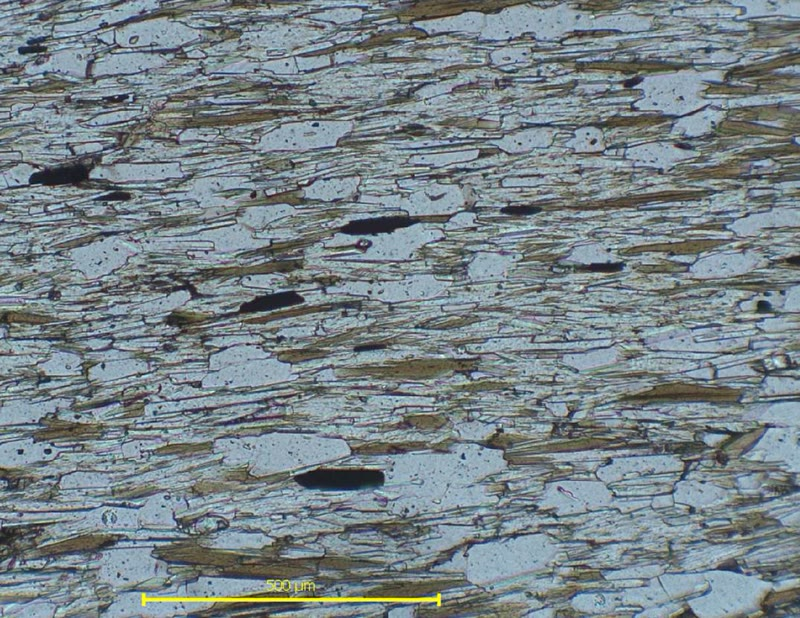
\includegraphics[height=4.3cm]{images/book2/g12-geoloshe-slaty-cleavage.jpg}\hspace{0.03\linewidth}%
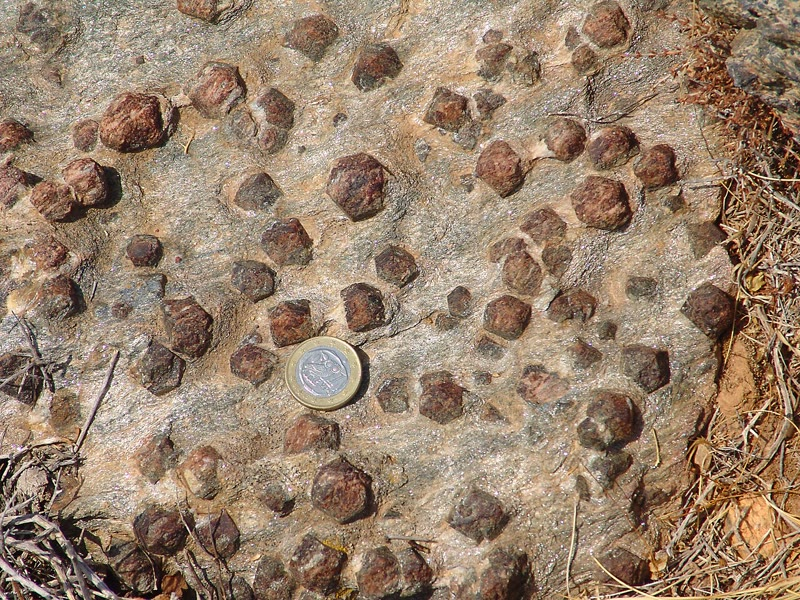
\includegraphics[height=4.3cm]{images/book2/g12-churchard-syros-garnet-schist.jpg}

\smallskip
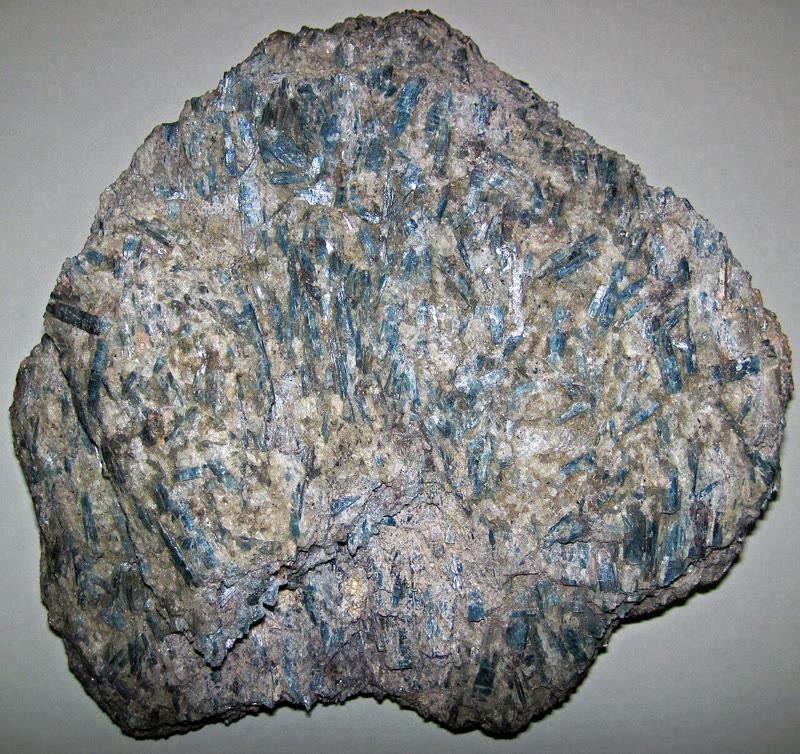
\includegraphics[height=4.3cm]{images/book2/g12-stjohn-kyanite-schist.jpg}\hspace{0.03\linewidth}%
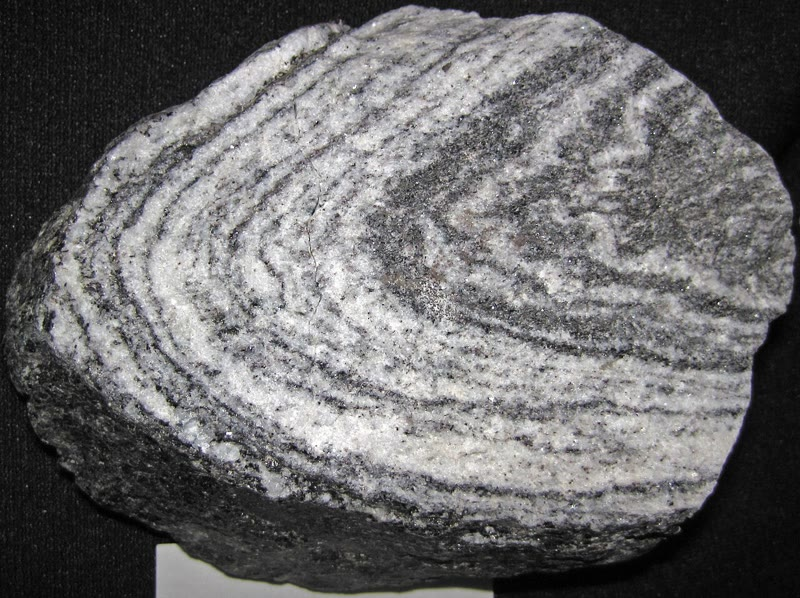
\includegraphics[height=4.3cm]{images/book2/g12-stjohn-gneiss.jpg}

{\small Arriba a la izquierda: una pizarra al microscopio (la barra amarilla
mide \qty{500}{\micro\metre}): sus escamas de mica están todas orientadas
igual. Arriba a la derecha: un esquisto micáceo con granates en la isla de
Siros; la moneda mide \qty{23}{mm} de diámetro. Abajo a la izquierda: un
esquisto con láminas azules de cianita. Abajo a la derecha: un gneis con
bandas de cuarzo (claras) y de mica biotita (oscuras). Fotografías de
Geoloshe (CC0), Graeme Churchard (CC~BY~2.0) y James St.~John (CC~BY~2.0).}
\end{omfigure}
% ledger: photo:g12-slaty-cleavage, photo:g12-syros-schist, photo:g12-kyanite-schist, photo:g12-gneiss

A lo largo de una \omterm{def:g11:lithosphere-asthenosphere:geotherm}{geoterma} típica, la pizarra se forma entre unos 5 y
\qty{10}{km} de profundidad, la filita entre 10 y 15, el esquisto entre 15 y
20, y el gneis entre 20 y \qty{25}{km}; más abajo aún, la roca empieza a
fundirse en algunos puntos. La \omterm{def:g12:metamorphic-rocks:foliation}{foliación} registra la dirección de la
compresión: se forma perpendicular al \omterm{def:g12:mountain-building:shortening}{acortamiento} que levanta las montañas
(el \cref{ch:g12:mountain-building}), y la estratificación original del fango
puede verse aún cortándola en ángulo.
% ledger: earle:settings, earle:foliation

Las rocas sin minerales planos o alargados no muestran \omterm{def:g12:metamorphic-rocks:foliation}{foliación} aunque se
compriman. Una caliza se convierte en un \textbf{mármol}, formado por
cristales de calcita más grandes en los que los fósiles se han borrado; una
arenisca se convierte en una \textbf{cuarcita}, cuyos granos de cuarzo han
crecido unos dentro de otros; y un fango calentado sin ser comprimido se
convierte en una roca dura, de grano fino y sin \omterm{def:g12:metamorphic-rocks:foliation}{foliación}, una
\textbf{corneana}.
% ledger: earle:foliation, earle:contact

\section{Metamorfismo de contacto y metamorfismo regional}

\begin{definition}[Metamorfismo de contacto; metamorfismo regional; aureola]\label{def:g12:metamorphic-rocks:contact-regional}
El \emph{metamorfismo de contacto}\index{metamorfismo de contacto} es el
\omterm{def:g12:metamorphic-rocks:metamorphism}{metamorfismo} de las rocas calentadas por un cuerpo de magma que se ha
introducido en ellas; se limita a una zona alrededor de la \omterm{def:g11:igneous-rocks:intrusion}{intrusión}, su
\emph{aureola}\index{aureola}, en la que el grado aumenta hacia el contacto.
El \emph{metamorfismo
regional}\index{metamorfismo regional} afecta a rocas enterradas a gran
profundidad en regiones extensas, normalmente donde convergen placas; las
rocas se comprimen además de calentarse, y casi siempre están foliadas.
\end{definition}
% ledger: earle:contact, earle:regional, tulane:metamorphism

\subsection{Alrededor de un cuerpo de magma}

Un cuerpo de magma a unos \qty{1000}{\celsius} que asciende hasta la fría
corteza superior calienta las rocas que lo rodean. Su temperatura puede
alcanzar de 300 a más de \qty{800}{\celsius}, a las bajas presiones de las
profundidades someras. La \omterm{def:g12:metamorphic-rocks:contact-regional}{aureola} es estrecha: unos centímetros alrededor de
una lámina fina de magma, hasta varias decenas de metros alrededor de un
cuerpo grande. Sus rocas se calientan sin comprimirse, así que no están
foliadas: el fango se convierte en corneana, la caliza en mármol, la arenisca
en cuarcita. Un cuerpo de magma que se instala a gran profundidad, en rocas
que ya están calientes, apenas forma \omterm{def:g12:metamorphic-rocks:contact-regional}{aureola}.
% ledger: earle:contact, earle:settings (magma bodies around 1000 degC)

\begin{omfigure}
\begin{tikzpicture}[font=\scriptsize]
  \def\pluton{(3.0,0) .. controls (3.0,2.3) and (7.0,2.3) .. (7.0,0) -- cycle}
  \def\aureole{(2.45,0) .. controls (2.45,2.95) and (7.55,2.95) .. (7.55,0) -- cycle}
  \fill[lith sandstone] (0,0) rectangle (10,0.8);
  \fill[lith limestone] (0,0.8) rectangle (10,1.6);
  \fill[lith shale] (0,1.6) rectangle (10,3);
  \fill[omThm, opacity=0.30] \aureole;
  \draw[omThm, line width=0.6pt, dashed] (2.45,0) .. controls (2.45,2.95) and (7.55,2.95) .. (7.55,0);
  \fill[lith granite] \pluton;
  \draw[black!70, line width=0.6pt] (3.0,0) .. controls (3.0,2.3) and (7.0,2.3) .. (7.0,0);
  \draw[black!60] (0,0) rectangle (10,3);
  \node[fill=white, inner sep=1.5pt] at (5,0.45) {granito (antes magma)};
  \draw[black!70] (6.0,1.95) -- (10.6,2.4) node[right] {corneana, a partir de fango};
  \draw[black!70] (7.0,1.2) -- (10.6,1.2) node[right] {mármol, a partir de caliza};
  \draw[black!70] (7.25,0.4) -- (10.6,0.4) node[right] {cuarcita, a partir de arenisca};
  \node[left] at (0,2.3) {lutita};
  \node[left] at (0,1.2) {caliza};
  \node[left] at (0,0.4) {arenisca};
  \draw[omThm] (4.2,2.05) -- (3.4,3.25) node[above, omThm] {aureola};
\end{tikzpicture}

{\small \omterm{def:g12:metamorphic-rocks:contact-regional}{Metamorfismo de contacto}, en corte: un cuerpo de magma ha ascendido
entre rocas sedimentarias estratificadas y ha calentado a su alrededor una
\omterm{def:g12:metamorphic-rocks:contact-regional}{aureola} estrecha (en rojo), cuyas rocas recristalizan sin ser comprimidas.
Esquema: las \omterm{def:g12:metamorphic-rocks:contact-regional}{aureolas} reales miden de centímetros a decenas de metros.}
\end{omfigure}
% ledger: earle:contact

\subsection{Bajo un cinturón montañoso}

El \omterm{def:g12:metamorphic-rocks:contact-regional}{metamorfismo regional} exige un enterramiento de 10 o \qty{20}{km}, así que
afecta a la vez a miles de kilómetros cuadrados. El lugar más probable es la
\omterm{def:g12:continental-crust:root}{raíz} de un cinturón montañoso, donde la colisión engrosa la corteza y empuja
sus rocas hacia abajo (el \cref{ch:g12:mountain-building}). En un antiguo
cinturón cuyas zonas se han cartografiado, las rocas de la zona de la
sillimanita se calentaron por encima de \qty{700}{\celsius} y se enterraron a
20 a \qty{25}{km} de profundidad, mientras que las de la zona exterior de la
clorita probablemente nunca se enterraron a más de unos \qty{5}{km}. Las
montañas de encima se desgastaron después a lo largo de decenas de millones de
años; al eliminarse la carga, la corteza gruesa volvió a subir, y las zonas
que estuvieron a gran profundidad afloran hoy en la superficie
(el \cref{ch:g12:destruction-of-mountains}).
% ledger: earle:regional

\subsection{Tres geotermas}

Los \omterm{def:g12:metamorphic-rocks:polymorph}{polimorfos} muestran de un vistazo que la misma profundidad no significa la
misma roca en todas partes: depende de la \omterm{def:g11:lithosphere-asthenosphere:geotherm}{geoterma}. La figura de los
\omterm{def:g12:metamorphic-rocks:polymorph}{polimorfos} lleva tres de ellas.
% ledger: earle:settings

\begin{itemize}
  \item Una \omterm{def:g11:lithosphere-asthenosphere:geotherm}{geoterma} \textbf{típica}, de unos \qty{30}{\celsius} por
        kilómetro: la temperatura alcanza unos \qty{300}{\celsius} a
        \qty{10}{km}. Pasa por debajo del punto triple, así que la cianita da
        paso directamente a la sillimanita, a unos \qty{574}{\celsius} y
        \qty{18.8}{km}.
  \item Una \omterm{def:g11:lithosphere-asthenosphere:geotherm}{geoterma} de \textbf{zona volcánica}, de 40 a \qty{50}{\celsius}
        por kilómetro, empinada por el calor del magma que asciende: las rocas
        alcanzan temperaturas altas a poca profundidad. A \qty{50}{\celsius}
        por kilómetro, la andalucita aparece hacia los \qty{6.6}{km} y da paso a
        la sillimanita hacia los \qty{10.9}{km}, a \qty{553}{\celsius}.
  \item La \omterm{def:g11:lithosphere-asthenosphere:geotherm}{geoterma} de una \textbf{\omterm{def:g11:subduction-zones:subduction}{zona de subducción}}, de menos de
        \qty{10}{\celsius} por kilómetro: la \omterm{def:g11:ocean-ridges:oceanic-lithosphere}{corteza oceánica} arrastrada hacia
        abajo se mantiene varios cientos de grados más fría que el manto que la
        rodea. A \qty{36}{km} está solo a unos \qty{370}{\celsius}, en pleno
        campo de la cianita. Es el camino frío y de alta presión en el que el
        basalto se convierte en \omterm{def:g11:subduction-zones:eclogite}{esquisto azul} y luego en \omterm{def:g11:subduction-zones:eclogite}{eclogita}, hacia los
        \qty{35}{km}.
\end{itemize}
% values: cross_30_0 573.6 degC 18.79 km; cross_50_0 340.1 degC 6.60 km; cross_50_1 553.0 degC 10.86 km; sub10_T_at_1gpa 370.2 (al2sio5.py)
% ledger: earle:settings

Así, cada roca metamórfica lleva un registro de la \omterm{def:g11:lithosphere-asthenosphere:geotherm}{geoterma} bajo la que se
formó, y del contexto de placas que había detrás: la andalucita y las
corneanas indican calor a poca profundidad, alrededor de cuerpos de magma; los
esquistos y gneises con cianita y sillimanita, las raíces profundas de los
cinturones montañosos; los \omterm{def:g11:subduction-zones:eclogite}{esquistos azules} y las \omterm{def:g11:subduction-zones:eclogite}{eclogitas}, las \omterm{def:g11:subduction-zones:subduction}{zonas de
subducción}. La mayoría de estas rocas solo se pueden ver porque volvieron a
la superficie sin transformarse de nuevo. Al ascender y enfriarse, sus
reacciones se frenan, y el agua que necesitarían las reacciones inversas se
escapó durante el descenso.
% ledger: earle:settings, earle:contact, tulane:metamorphism (retrograde metamorphism uncommon)

\section{Ejercicios}

\begin{exercise}[$\star$]\label{exo:g12:metamorphic-rocks:1}
Da la palabra: (a) minerales con la misma composición pero estructuras
cristalinas distintas; (b) la línea de un mapa donde aparece por primera vez
un \omterm{def:g12:metamorphic-rocks:index-mineral}{mineral índice}; (c) la zona de rocas calentadas alrededor de un cuerpo de
magma; (d) los planos paralelos que forman los minerales planos alineados;
(e) la presión debida al peso de las rocas de encima.
\end{exercise}

\begin{exercise}[$\star$]\label{exo:g12:metamorphic-rocks:2}
Nombra la roca metamórfica en que se convierte cada roca original: (1) una
caliza; (2) una arenisca; (3) un fango, a grado bajo y comprimido; (4) un
fango, a grado alto; (5) un fango, calentado por un cuerpo de magma sin ser
comprimido.
\end{exercise}

\begin{exercise}[$\star$]\label{exo:g12:metamorphic-rocks:3}
Con $\rho = \qty{2830}{kg/m^3}$ y $g = \qty{9.81}{m/s^2}$, calcula la
\omterm{def:g12:metamorphic-rocks:lithostatic}{presión litostática}, en \unit{GPa}, a \qty{10}{km} y a \qty{20}{km}.
\end{exercise}

\begin{exercise}[$\star$]\label{exo:g12:metamorphic-rocks:4}
En el diagrama de los \omterm{def:g12:metamorphic-rocks:polymorph}{polimorfos} de \ce{Al2SiO5}, ¿qué mineral es estable
(1) a \qty{400}{\celsius} y \qty{0.6}{GPa}; (2) a \qty{500}{\celsius}
y \qty{0.2}{GPa}; (3) a \qty{750}{\celsius} y \qty{0.3}{GPa}?
\end{exercise}

\begin{exercise}[$\star$]\label{exo:g12:metamorphic-rocks:5}
(1) Ordena de menor a mayor grado: esquisto, pizarra, gneis, filita. (2) ¿En
cuál de ellas se ven las micas a simple vista? (3) ¿Cuál muestra bandas
claras y oscuras?
\end{exercise}

\begin{exercise}[$\star\star$]\label{exo:g12:metamorphic-rocks:6}
(1) Calcula la \omterm{def:g12:metamorphic-rocks:lithostatic}{presión litostática} en la base de una corteza de \qty{35}{km}
de espesor ($\rho = \qty{2830}{kg/m^3}$) y exprésala en atmósferas
($\qty{1}{atm} = \qty{101325}{Pa}$). (2) Calcula la presión en el fondo
de un océano de \qty{4}{km} de profundidad, con agua de mar de densidad
\qty{1025}{kg/m^3}. (3) ¿Cuántas veces mayor es la primera?
\end{exercise}

\begin{exercise}[$\star\star$]\label{exo:g12:metamorphic-rocks:7}
El punto triple del \ce{Al2SiO5} está a \qty{504}{\celsius} y
\qty{0.375}{GPa}. (1) ¿A qué profundidad se alcanza esa presión ($\rho =
\qty{2830}{kg/m^3}$)? (2) ¿Qué \omterm{def:g11:lithosphere-asthenosphere:geotherm}{gradiente geotérmico}, partiendo de
\qty{10}{\celsius} en la superficie, pasa exactamente por él? (3) ¿Es probable
que sea común una roca que contenga los tres \omterm{def:g12:metamorphic-rocks:polymorph}{polimorfos}?
\end{exercise}

\begin{exercise}[$\star\star$]\label{exo:g12:metamorphic-rocks:8}
En la fotografía del esquisto con granates de Siros, los granates mayores
miden alrededor de un tercio del diámetro de la moneda, que es de
\qty{23}{mm}. (1) Estima su diámetro. (2) Si el diámetro de un granate crece
alrededor de \qty{1}{mm} en un millón de años, ¿cuánto tardaron en crecer?
(3) ¿Qué te dice eso sobre el tiempo que pasa una roca en profundidad?
\end{exercise}

\begin{exercise}[$\star\star$]\label{exo:g12:metamorphic-rocks:9}
Al recorrer \qty{24}{km} hacia el oeste a través de un antiguo cinturón
montañoso, un geólogo registra rocas formadas a partir de fango. Al principio
solo contienen clorita y biotita; el primer granate aparece a los
\qty{6}{km}, la primera estaurolita a los \qty{11}{km}, la primera cianita a
los \qty{15}{km} y la primera sillimanita a los \qty{20}{km}. (1) ¿Cuántas
\omterm{def:g12:metamorphic-rocks:index-mineral}{isógradas} se han cruzado? Nómbralas en orden. (2) ¿En qué dirección aumenta
el grado? (3) ¿Dónde se enterraron más las rocas, y aproximadamente qué
temperatura alcanzaron allí?
\end{exercise}

\begin{exercise}[$\star\star$]\label{exo:g12:metamorphic-rocks:10}
Un cuerpo de magma asciende entre capas de fango, caliza y arenisca cerca de
la superficie. (1) Nombra la roca en que se convierte cada capa junto a él.
(2) ¿Por qué estas rocas no están foliadas? (3) Un segundo cuerpo de magma se
instala a \qty{20}{km} de profundidad, en rocas que ya están cerca de
\qty{500}{\celsius}. ¿Por qué apenas forma \omterm{def:g12:metamorphic-rocks:contact-regional}{aureola}?
\end{exercise}

\begin{exercise}[$\star\star$]\label{exo:g12:metamorphic-rocks:11}
Una capa de fango se comprime desde el este y el oeste durante una colisión,
y forma micas al calentarse. (1) ¿Cómo se orientan las micas: con sus caras
planas mirando al este--oeste o al norte--sur? (2) ¿La \omterm{def:g12:metamorphic-rocks:foliation}{foliación} que se forma
es horizontal o vertical? (3) Un mármol y una cuarcita comprimidos del mismo
modo no muestran \omterm{def:g12:metamorphic-rocks:foliation}{foliación}. ¿Por qué?
\end{exercise}

\begin{exercise}[$\star\star\star$]\label{exo:g12:metamorphic-rocks:12}
Entre 500 y \qty{700}{\celsius}, el límite cianita--sillimanita se aproxima a
la recta $P = 0.577 + 0.00209\,(T - 600)$, con $P$ en
\unit{GPa} y $T$ en \unit{\celsius}. Una \omterm{def:g11:lithosphere-asthenosphere:geotherm}{geoterma} típica es $T = 10 + 30z$
($z$ en \unit{km}), y $P = 0.0278\,z$. (1) Escribe la \omterm{def:g11:lithosphere-asthenosphere:geotherm}{geoterma} como $P$ en
función de $T$. (2) Halla dónde cruza el límite: temperatura, presión,
profundidad. (3) A lo largo de esta \omterm{def:g11:lithosphere-asthenosphere:geotherm}{geoterma}, ¿qué \omterm{def:g12:metamorphic-rocks:polymorph}{polimorfo} es estable justo
por encima de esa profundidad, y cuál justo por debajo?
\end{exercise}

\begin{exercise}[$\star\star\star$]\label{exo:g12:metamorphic-rocks:13}
(1) A lo largo de una \omterm{def:g11:lithosphere-asthenosphere:geotherm}{geoterma} de \omterm{def:g11:subduction-zones:subduction}{subducción} de \qty{10}{\celsius} por
kilómetro, partiendo de \qty{10}{\celsius}, ¿cuál es la temperatura a
\qty{35}{km}, donde se forma la \omterm{def:g11:subduction-zones:eclogite}{eclogita}? (2) ¿Cuál es a lo largo de una
\omterm{def:g11:lithosphere-asthenosphere:geotherm}{geoterma} típica de \qty{30}{\celsius} por kilómetro? (3) Sitúa los dos puntos
en el diagrama de los \omterm{def:g12:metamorphic-rocks:polymorph}{polimorfos}: ¿qué \omterm{def:g12:metamorphic-rocks:polymorph}{polimorfo} es estable en el primero?
(4) ¿Por qué los \omterm{def:g11:subduction-zones:eclogite}{esquistos azules} y las \omterm{def:g11:subduction-zones:eclogite}{eclogitas} se forman en las \omterm{def:g11:subduction-zones:subduction}{zonas de
subducción} y casi en ningún otro lugar?
\end{exercise}

\begin{exercise}[$\star\star\star$]\label{exo:g12:metamorphic-rocks:14}
Las densidades de la cianita, la sillimanita y la andalucita son \num{3.61},
\num{3.24} y \qty{3.15}{g/cm^3}. (1) Calcula el volumen de \qty{1}{kg} de
cada una, en \unit{cm^3}. (2) ¿En qué porcentaje es la cianita más pequeña que
la andalucita de la misma masa? (3) Explica, con la idea de que una presión
alta favorece la disposición que ocupa menos espacio, por qué la cianita ocupa
el campo de alta presión del diagrama.
\end{exercise}

\begin{exercise}[$\star\star\star$]\label{exo:g12:metamorphic-rocks:15}
En un antiguo cinturón montañoso, las rocas de la zona de la sillimanita se
calentaron por encima de \qty{700}{\celsius} y se enterraron a 20 a
\qty{25}{km} de profundidad. (1) Calcula la presión a 20 y a \qty{25}{km}.
(2) Con la recta del ejercicio~12, halla la temperatura más baja a la que la
sillimanita es estable a cada una de esas presiones. ¿Es \qty{700}{\celsius}
compatible con la sillimanita? (3) ¿Qué \omterm{def:g11:lithosphere-asthenosphere:geotherm}{gradientes geotérmicos}, partiendo de
\qty{10}{\celsius} en la superficie, implican \qty{700}{\celsius} a 20 y a
\qty{25}{km}? (4) Las rocas quedaron expuestas en la superficie unos 40
millones de años después. ¿A qué ritmo medio se eliminó la roca que tenían
encima, en \unit{mm} al año?
\end{exercise}

\begin{problem}[{Problema de fin de semana --- La historia de un esquisto con cianita}]
\label{pb:g12:metamorphic-rocks:1}
% ledger: hm93:table11, cm95:crust, earle:controls, earle:settings, earle:regional, tulane:roots, tulane:metamorphism, iugs:barrow; Book 3: webmineral:polymorphs; Book 1: ussa76:sea-level
% values: pb_z_km 25.214, pb_grad 23.4, pb_kysil_P_at_600_gpa 0.577 (al2sio5.py); t_on_kysil(7.0) = 658.9
Un esquisto recogido en el núcleo de un antiguo cinturón montañoso contiene
moscovita, biotita, cuarzo, granates de hasta \qty{8}{mm} de diámetro y
láminas azules de cianita; no contiene ni sillimanita ni andalucita. Los
análisis de laboratorio de su granate y su biotita dan las condiciones en las
que cristalizó: unos \qty{600}{\celsius} y \qty{0.70}{GPa}. Toma $\rho =
\qty{2830}{kg/m^3}$, $g = \qty{9.81}{m/s^2}$, \qty{10}{\celsius} en la
superficie, y la recta cianita--sillimanita del ejercicio~12, $P = 0.577 +
0.00209\,(T - 600)$.

\medskip
\noindent\textbf{Parte I --- Los minerales.}
\begin{enumerate}
  \item ¿Por qué se llama esquisto a esta roca? ¿Cuáles de sus minerales
        forman la \omterm{def:g12:metamorphic-rocks:foliation}{esquistosidad}?
  \item La cianita, la andalucita y la sillimanita comparten una fórmula.
        Escríbela, y da la palabra que designa a esos minerales.
  \item Las densidades de la cianita y la andalucita son \num{3.61} y
        \qty{3.15}{g/cm^3}. ¿En qué porcentaje es menor el volumen de un
        kilogramo de cianita? ¿Cuál de las dos favorece la presión?
  \item En la secuencia de \omterm{def:g12:metamorphic-rocks:index-mineral}{minerales índice} de las rocas formadas a partir de
        fango, ¿a qué zona pertenece la roca? ¿Qué \omterm{def:g12:metamorphic-rocks:index-mineral}{isógradas} cruzó en su descenso?
  \item Si el diámetro de los granates creció alrededor de \qty{1}{mm} en un
        millón de años, ¿cuánto tardaron en crecer los mayores?
\end{enumerate}

\medskip
\noindent\textbf{Parte II --- Presión y temperatura.}
\begin{enumerate}[resume]
  \item A \qty{600}{\celsius}, ¿por encima de qué presión es estable la
        cianita en lugar de la sillimanita?
  \item Comprueba que el punto (\qty{600}{\celsius}, \qty{0.70}{GPa}) está en
        el campo de la cianita.
  \item La ausencia de sillimanita da una presión mínima a
        \qty{600}{\celsius}. ¿Cuál es?
  \item Si la roca se hubiera calentado más a \qty{0.70}{GPa}, ¿a qué
        temperatura se habría transformado su cianita en sillimanita?
  \item Expresa \qty{0.70}{GPa} en kilobares ($\qty{1}{kbar} =
        \qty{e8}{Pa}$) y en atmósferas ($\qty{1}{atm} = \qty{101325}{Pa}$).
\end{enumerate}

\medskip
\noindent\textbf{Parte III --- La profundidad de enterramiento.}
\begin{enumerate}[resume]
  \item ¿Cuántos megapascales aumenta la \omterm{def:g12:metamorphic-rocks:lithostatic}{presión litostática} por
        kilómetro?
  \item ¿A qué profundidad estaba el esquisto cuando cristalizó?
  \item ¿Cuál es la profundidad mínima que permite la ausencia de
        sillimanita (pregunta 8)?
  \item Rehaz la pregunta 12 con una densidad de \qty{2700}{kg/m^3} para las
        rocas de encima. ¿En qué porcentaje cambia la profundidad?
  \item Una \omterm{def:g12:continental-crust:continental-crust}{corteza continental} tiene normalmente de 35 a \qty{40}{km} de
        espesor, y de 50 a \qty{70}{km} bajo los cinturones montañosos.
        ¿Cristalizó el esquisto en la corteza o en el manto?
\end{enumerate}

\medskip
\noindent\textbf{Parte IV --- La geoterma y el camino de vuelta.}
\begin{enumerate}[resume]
  \item ¿Qué \omterm{def:g11:lithosphere-asthenosphere:geotherm}{gradiente geotérmico} medio implican \qty{600}{\celsius} a esa
        profundidad?
  \item Compáralo con los gradientes de una \omterm{def:g11:subduction-zones:subduction}{zona de subducción}, de una
        corteza típica y de una zona volcánica. ¿Qué tipo de \omterm{def:g12:metamorphic-rocks:metamorphism}{metamorfismo}
        formó la roca?
  \item A lo largo de una \omterm{def:g11:lithosphere-asthenosphere:geotherm}{geoterma} típica de \qty{30}{\celsius} por
        kilómetro, ¿cuál sería la temperatura a la profundidad de la
        pregunta 12? ¿Qué \omterm{def:g12:metamorphic-rocks:polymorph}{polimorfo} sería entonces estable a \qty{0.70}{GPa}?
  \item Para traer el esquisto a la superficie, hubo que eliminar toda la
        roca que tenía encima. A un ritmo medio de \qty{0.5}{mm} al año,
        ¿cuánto tiempo hizo falta?
  \item ¿Por qué la cianita no volvió a transformarse en andalucita durante
        el ascenso?
  \item En resumen: ¿a qué profundidad cristalizó este esquisto con cianita?
\end{enumerate}
\end{problem}
